\documentclass [portrait,a0, 25pt]{a0poster}

\usepackage{theoposter_tudo}	% Do explicitly use the local version of theoposter.sty
\usepackage{xspace}
\usepackage{fontawesome}	% icons

% MRW Packages
\usepackage{multicol}
\usepackage{bm}
\usepackage{braket}
\usepackage{dsfont}
\usepackage{siunitx}
\usepackage{nicefrac}

\usepackage[mode=buildnew]{standalone}% requires -shell-escape

\newcommand{\im}{\mathrm{i}}

\newcommand{\highlightNat}[1]{\textbf{\textcolor{tugreen}{#1}}}
\newcommand{\highlightDarkNat}[1]{\textbf{\textcolor{tudarkgreen}{#1}}}

\newcommand{\highlightOne}[1]{\highlightNat{#1}}

\newcommand{\ddt}{\frac{\mathrm{d}}{\mathrm{d}t}}
\newcommand{\dgamma}{\mathrm{d}\gamma}

\newcommand{\mM}{\mathcal{M}}
\newcommand{\mN}{\mathcal{N}}

\newcommand{\greens}[1]{\mathcal{G}_\text{#1} (\omega)}
\newcommand{\spectral}[1]{\mathcal{A}_\text{#1}  (\omega)}


% For more tikz
\usetikzlibrary{arrows.meta}


\begin{document}%
\fontsize{22}{22} % 10pt is the standard size

\begin{tikzpicture}[overlay, inner sep=0pt, outer sep=0pt]
	\posterhead%
		{ % title
        Collective excitations in competing phases \\ in two and three dimensions
        }
		{ % authors % set a normal space after an abbreviation, instead of an inter-sentence space
            \underline{Joshua Alt\"user}\textsuperscript{1},
            Götz S.\ Uhrig\textsuperscript{1},
        }	% underline the name of the presenting author
		{ % affiliations
            \textsuperscript{1}Condensed Matter Theory, Technische Universität Dortmund, Otto-Hahn-Str.\ 4, 44227 Dortmund, Germany\\
		}
\newcommand*\TikZ{Ti\textit{k}Z\xspace}


\posterbox{2cm}{26cm}{38cm}{Introduction}
{%
\begin{itemize}
    \item Study of collective behavior of many particles rather than individual ones
    \item Complex interplay of various degrees of freedom
    \item Governs many structural, magnetic, and electronic phenomena
\end{itemize}

\highlightOne{ Investigated phases } \\
\begin{itemize}
    \item $s$-wave superconductivity (SC), Charge-density wave (CDW), and antiferromagnetism (AFM) (nesting vector $\vec{Q} = (\pi, \ldots)$)
\end{itemize}

\begin{minipage}{0.64\textwidth}
    \highlightOne{ Investigated excitations } \\
    \begin{itemize}
        \item (CDW) Exciton: $1/N \sum_{k} \left( g_{\vec{k}\uparrow} + g_{\vec{k}\downarrow} \right),\qquad g_{\vec{k}\sigma}$
        \item (AFM) Longitudinal magnon: $1/N \sum_{k} \left( g_{\vec{k}\uparrow} - g_{\vec{k}\downarrow} \right)$
        \item (AFM) Transversal magnon: $1/N \sum_{k} \left( \tau_{\vec{k}} + \tau_{\vec{k}}^\dagger \right)$
        \item (SC) Amplitude (Higgs) mode: $1/N \sum_{k} \left( f_{\vec{k}} + f_{\vec{k}}^\dagger \right)$
        \item (SC) Phase (Anderson-Bogoliubov) mode: $\im /N \sum_{k} \left( f_{\vec{k}} - f_{\vec{k}}^\dagger \right) $
    \end{itemize}
\end{minipage}
\hfill
\begin{minipage}{0.35\textwidth}
\highlightOne{ Abbreviations }
\begin{equation*}
    \label{eqn:operators}
    \begin{aligned}
        n_{k\sigma} &\coloneqq  c_{\vec{k}\sigma}^\dagger c_{\vec{k}\sigma}\,,          \\
        f_k     &\coloneqq  c_{-\vec{k}\downarrow} c_{\vec{k}\uparrow}\,, \\
        g_{k\sigma} &\coloneqq  c_{\vec{k}\sigma}^\dagger c_{\vec{k}+\vec{Q}\sigma}\,,  \\
        \tau_k  &\coloneqq  c_{\vec{k}\uparrow}^\dagger c_{\vec{k}\downarrow}\,,
    \end{aligned}
\end{equation*}
\end{minipage}
}

\posterbox{2cm}{45cm}{38cm}{Method: Iterated equations of motion (iEoM) \cite{Kalthoff17,Bleicker18}}
{%
\highlightOne{ Key ideas }
\begin{itemize}
\item Consider a time-dependent operator $\hat{a}(t) = \sum_j c_j(t) \hat{A}_j$ and the symplectic product $(\hat{A} | \hat{B}) \coloneqq \langle [\hat{A}^\dagger, \hat{B}] \rangle$
\item Write the Heisenberg EoM as matrix-vector EoM
\begin{equation*}
    \label{eqn:heisenberg}
    \begin{aligned}
        \ddt \hat{a}(t) = \sum_j \ddt c_j(t) \hat{A}_j &= i \sum_j c_j(t) [H, \hat{A}_j] \\
        \Rightarrow \sum_j \underbrace{(\hat{A}_i | \hat{A}_j)}_{\coloneqq \mN_{ij}} \ddt c_j(t) &= i \sum_j \underbrace{(\hat{A}_i | [\hat{H}, \hat{A}_j])}_{\coloneqq \mM_{ij}} c_j(t) \\
        \Rightarrow \mN \ddt \vec{c}(t) &= i \mM \vec{c}(t)\,.
    \end{aligned}
\end{equation*}
\item Generalized eigenvalue problem $\omega \mN \vec{v} = \mM \vec{v}$, real solutions if either $\mM$ or $\mN$ is nonnegative.
\begin{itemize}
    \item $\mM$ is nonnegative is thermal equilibrium
\end{itemize}
\end{itemize}

\highlightOne{ Green's functions }
\begin{itemize}
    \item Elements of the matrix $\greens{ } \coloneqq \mN [-(\omega + \im 0^+) \mN - \mM]^{-1} \mN$ are Fourier-transformed Green's functions
    \item Specifically
    \begin{equation*}
        \mathcal{G}_{ij}(\omega) = G_{\hat{A}_i \hat{A}_j^\dagger} (\omega) = -\im \int_0^{\infty} \langle [A_i(t), A_j^\dagger(0)] \rangle e^{\im (\omega + \im 0^+) t} \mathrm{d}t
    \end{equation*}
    \item Lengthy calculations yield a quadratic form
    \begin{equation*}
        \frac{1}{-(\omega + \im 0^+) \mN - \mM} \to \check{N}^{-1/2} \frac{1}{(\omega + \im 0^+)^2 - \check{M}} \check{N}^{-1/2}
    \end{equation*}
    \item Matrix inverse by tridiagonalization and subsequent continued fraction expansion with square-root terminator
\end{itemize}
}

\posterbox{2cm}{72.5cm}{38cm}{Model}
{%
\begin{minipage}{0.59\textwidth}
    \highlightOne{ Hamiltonian: Extended Hubbard model }
    \begin{equation*}
        \label{eqn:full_hamiltonian}
        \begin{aligned}
            H = &-t \sum_{\langle i, j \rangle, \sigma} \left( c_{i\sigma}^\dagger c_{j\sigma} + \text{h.c.} \right) 
            + \mu \sum_{i,\sigma} n_{i\sigma} \\
            &+ U \sum_{i} n_{i\uparrow} n_{i\downarrow} 
            + \frac{V}{2} \sum_{\langle i, j\rangle, \sigma} n_{i\sigma} n_{j\sigma}\,,
        \end{aligned}
    \end{equation*}
    \begin{itemize}
        \item Half-filling, on both a square and a simple cubic lattice, temperature $T=0$
    \end{itemize}
    \highlightOne{ Static mean-field theory }
    \begin{itemize}
        \item Used to deal with the interaction terms and to obtain expectation values for iEoM
        \item Terms depend on $\hat{\gamma}(\vec{k}) \coloneqq \frac{1}{D} \sum_{\alpha=1}^D \cos(k_\alpha)$ \\
        $\Rightarrow$ DOS based description $\rho \coloneqq \frac{1}{N} \sum_{\vec{k}} \delta(\gamma - \hat{\gamma}(\vec{k}))$
        \begin{align*}
            \Delta_\text{CDW} &= \left(\frac{U}{2N} - \frac{zV}{N}\right) \sum_{\sigma} \int \langle g_{\sigma} (\gamma) \rangle \dgamma\\\ 
            \Delta_\text{SC} &= \frac{U}{N} \int \langle f(\gamma) \rangle \dgamma\\
            \Delta_\text{AFM} &= \frac{U}{2N} \int \left( \langle g_{\uparrow} (\gamma) \rangle - \langle g_{\downarrow} (\gamma) \rangle \right) \dgamma\\ 
            \Delta_n &= \frac{V}{N} \sum_{\sigma} \int \gamma \langle n_{\sigma} (\gamma) \rangle \dgamma
        \end{align*}
        \item Allows us to tackle both 2D and 3D systems
    \end{itemize}
\end{minipage}
\hfill
\begin{minipage}{0.4\textwidth}
    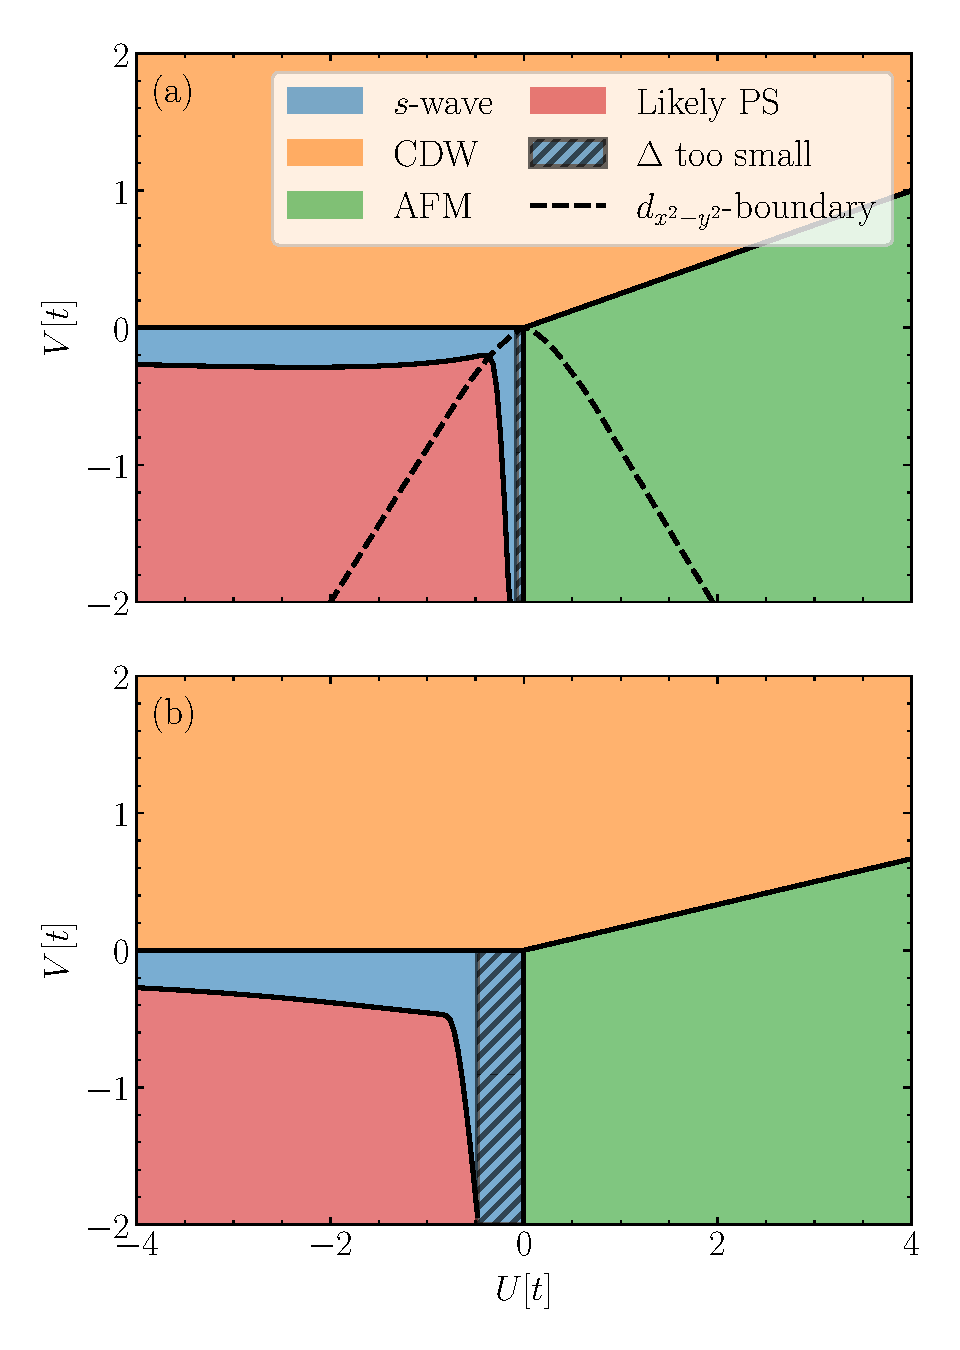
\includegraphics[width=\textwidth]{plots/phase_diagram.pdf}
    \center{\textcolor{tudarkgreen}{Mean-field phase diagram of the extended Hubbard model. 
    (a) Square lattice (b) simple cubic lattice. $d_{x^2-y^2}$ from Ref. \cite{Micnas88b}.}}
\end{minipage}
\highlightOne{ Phase diagram }
\begin{itemize}
    \item Mostly the same for both lattices, $d_{x^2 -y^2}$-wave SC for $V<0$ on the square lattice is inaccessible to us
    \item Red region: Mean-field self-consistency converges to $s$-wave SC, but $\mM$ is not nonnegative $\Rightarrow$ not the true groundstate.
    Literature suggests a phase-separated state. \cite{Linner23}
    \item Purple region: Inaccuracies due to finite discretization dominate; here the gap is of the same order of magnitude as our gap
\end{itemize}
}



\posterbox{42cm}{26cm}{38cm}{Spectral functions}
{%
\highlightOne{Close to SC-CDW phase transition} \\
\begin{minipage}{0.65\textwidth}
    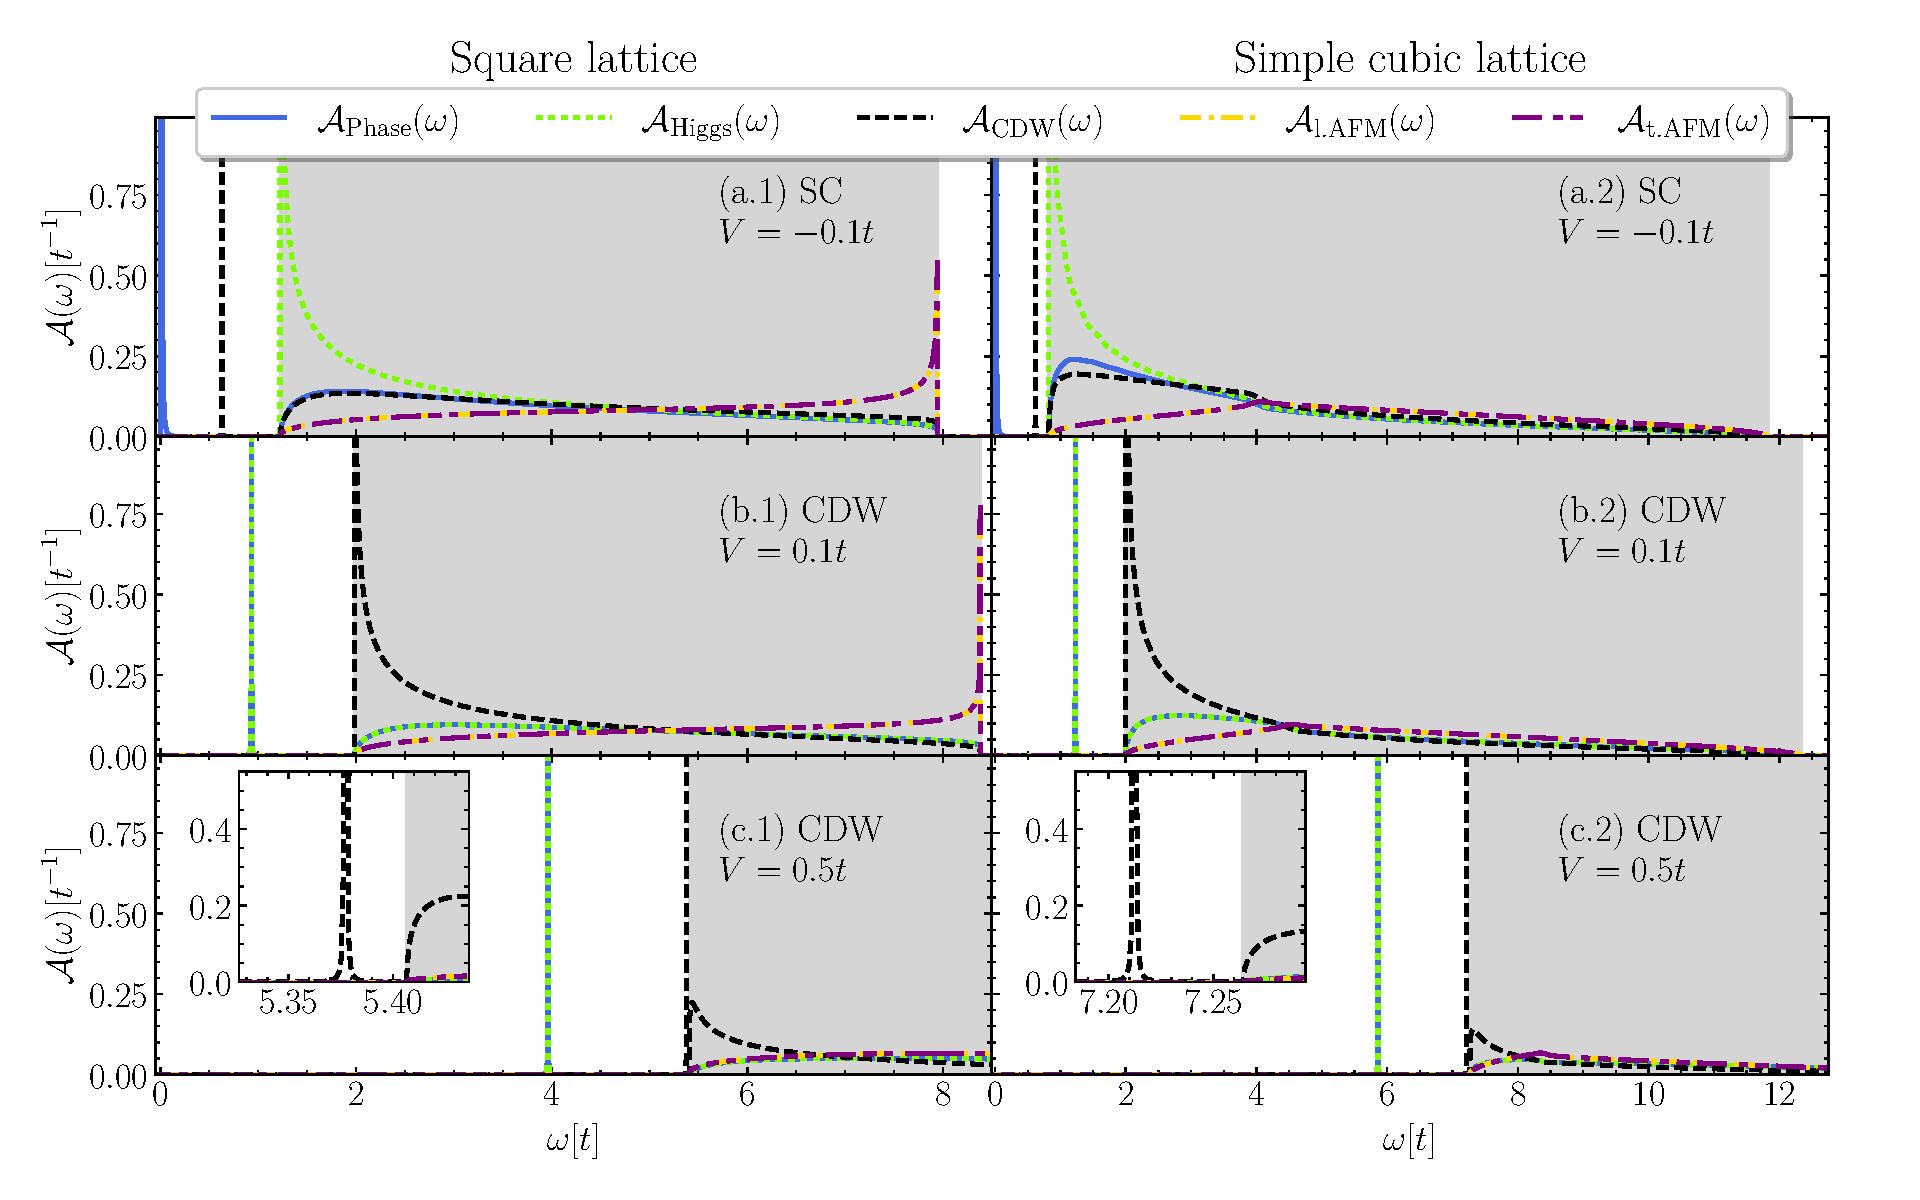
\includegraphics[width=\textwidth]{plots/resolvent_overview_SC_CDW.pdf} % NV sketch
\end{minipage}
\hfill
\begin{minipage}{0.34\textwidth}
    \begin{itemize}
        \item SC phase:
        \begin{itemize}
            \item Peak at $0$: Anderson-Bogoliubov mode, $\propto \delta'(\omega)$
            \item Singularity at $2\Delta$: Higgs mode, \\$\propto 1/\sqrt{\omega - 2\Delta}$
            \item CDW spectral function has a peak below the two-particle continuum
        \end{itemize}
        \item CDW phase:
        \begin{itemize}
            \item Phase and amplitude SC spectral functions are identical
            \item Both have a peak below the two-particle continuum
            \item For moderate $V$: singularity in the CDW spectral function, \\$\propto 1/\sqrt{\omega - 2\Delta}$
            \item For larger $V$: peak below the continuum
        \end{itemize}
    \end{itemize}
\end{minipage}

\highlightOne{CDW-SC coexistence at $V=0$} \\
\begin{minipage}{0.65\textwidth}
    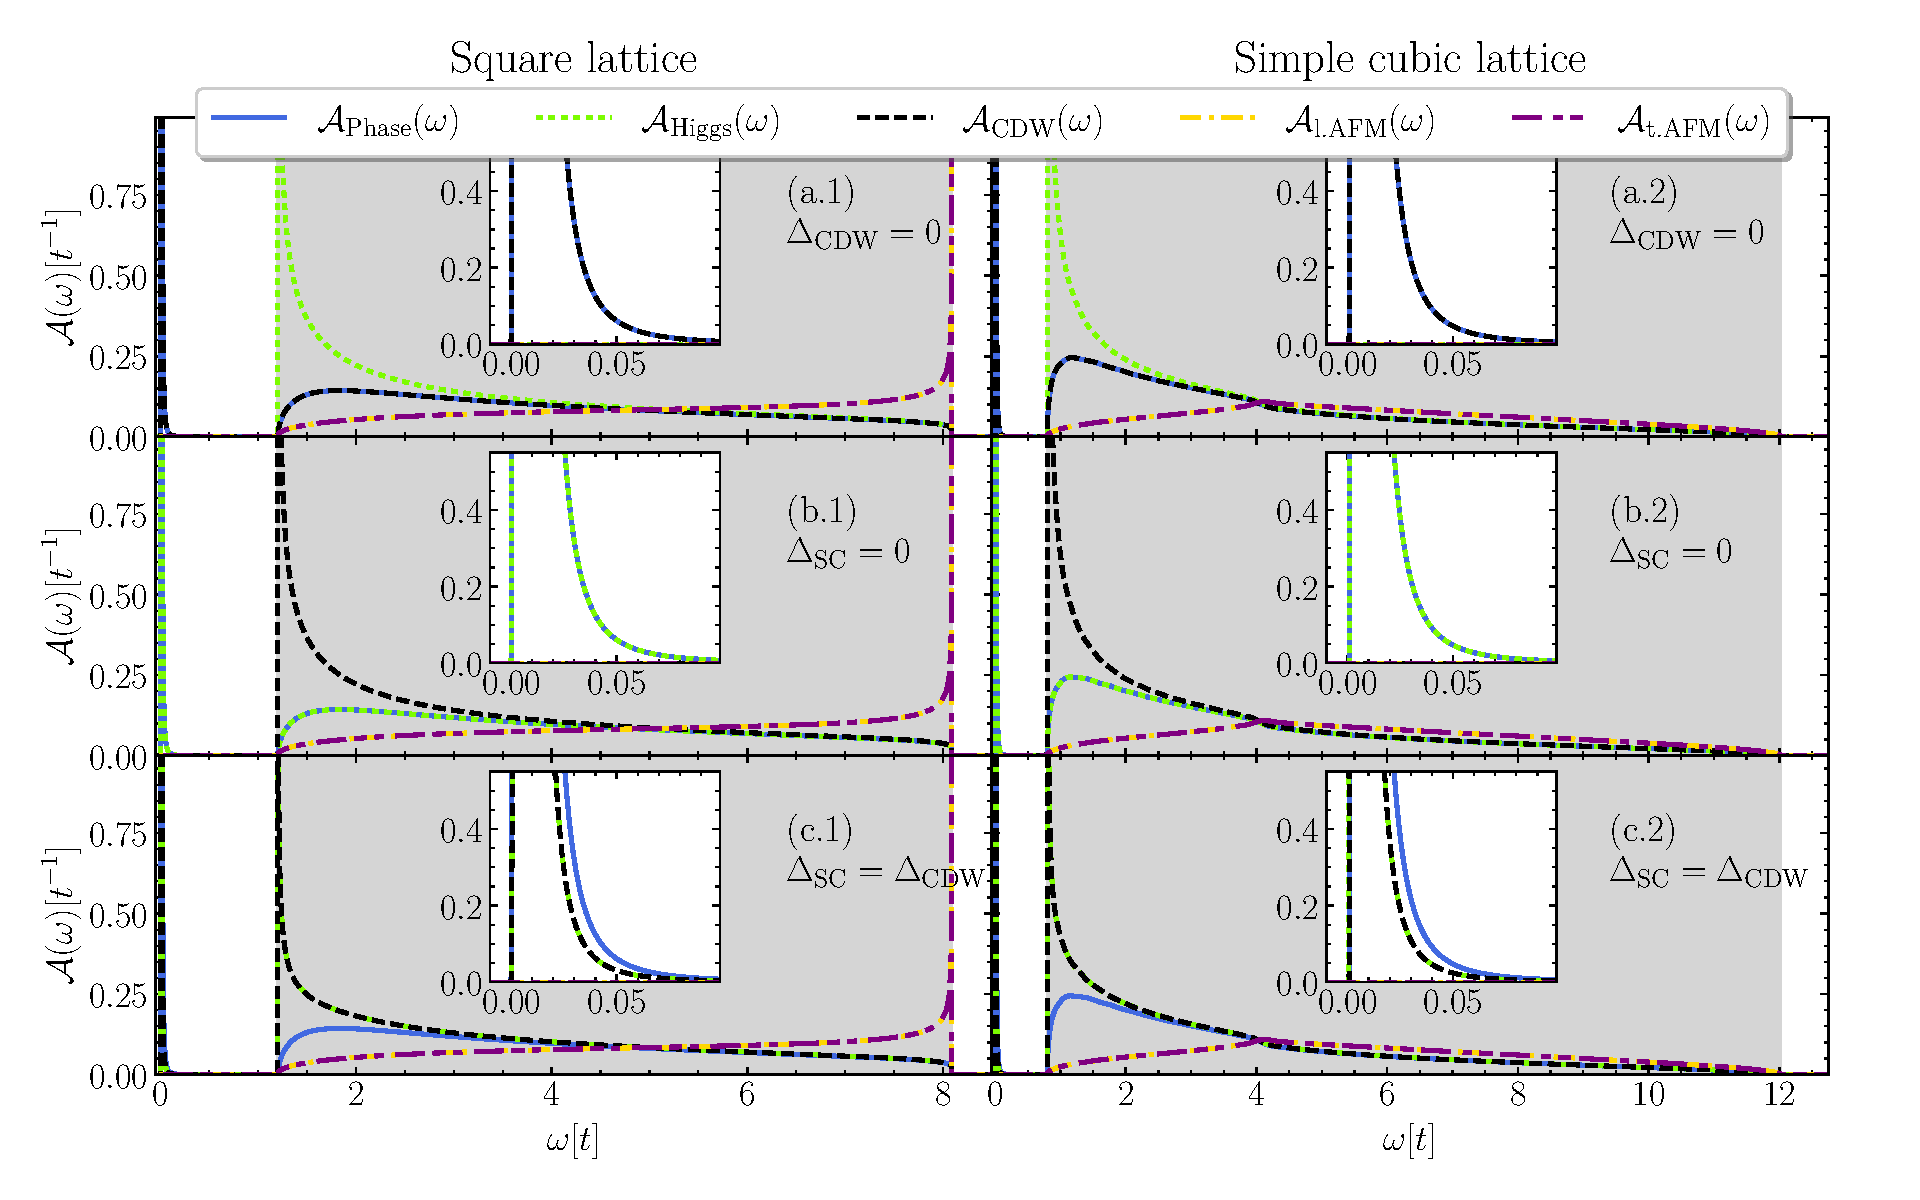
\includegraphics[width=\textwidth]{plots/resolvent_overview_V0.pdf} % NV sketch
\end{minipage}
\hfill
\begin{minipage}{0.34\textwidth}
    \begin{itemize}
        \item The ratio $\Delta_\text{CDW} / \Delta_\text{SC}$ may be chosen arbitrarily as long as $\Delta_\text{tot} \coloneqq \sqrt{\Delta_\text{CDW}^2 + \Delta_\text{SC}^2} = \text{const}$
        \item Anderson-Bogoliubov mode always exits
        \item For $\Delta_\text{CDW} = 0$, the Higgs mode exists at $\omega = 2\Delta_\text{tot}$, while the CDW spectral function has a peak at $\omega=0$
        \item The reverse applies for $\Delta_\text{SC} = 0$
        \item $\Delta_\text{CDW} = \Delta_\text{SC}$ yields a mixture of the two
    \end{itemize}
\end{minipage}

\highlightOne{Close to AFM-CDW phase transition} \\
\begin{minipage}{0.65\textwidth}
    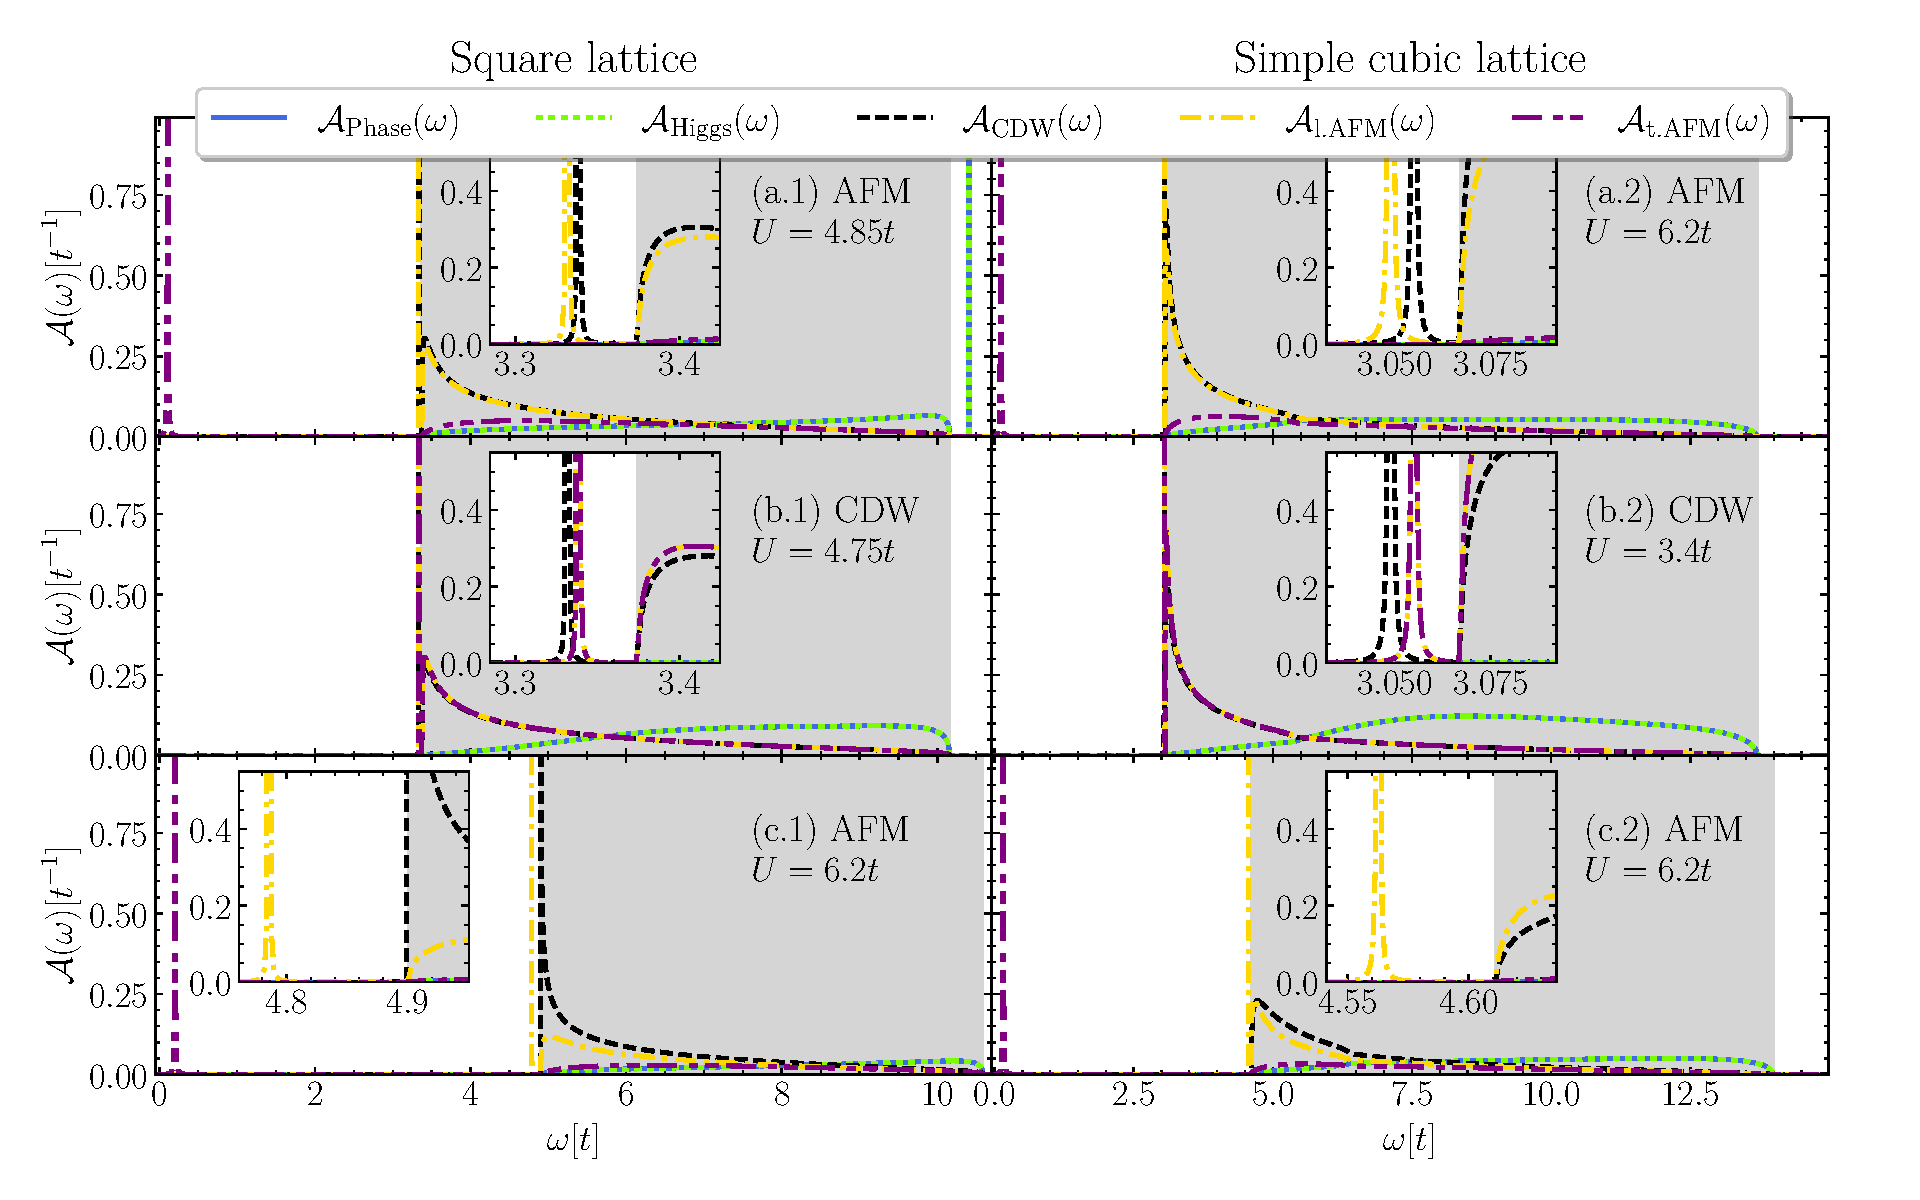
\includegraphics[width=\textwidth]{plots/resolvent_overview_AFM_CDW.pdf} % NV sketch
    \center{\textcolor{tudarkgreen}{Spectral functions for various collective excitations.}}
\end{minipage}
\hfill
\begin{minipage}{0.34\textwidth}
    \begin{itemize}
        \item AFM phase: Transversal AFM spectral function has a peak at $0$
        \item Longitudinal AFM spectral function behaves just like the CDW spectral function
        \item Close to the phase transition: Both have a peak below the continuum
        \item Further away: Only the spectral function corresponding to the phase has a peak below the continuum
    \end{itemize}
\end{minipage}
}

\posterbox{42cm}{78cm}{38cm}{Behavior of the peaks}
{%
\begin{minipage}{0.49\textwidth}
    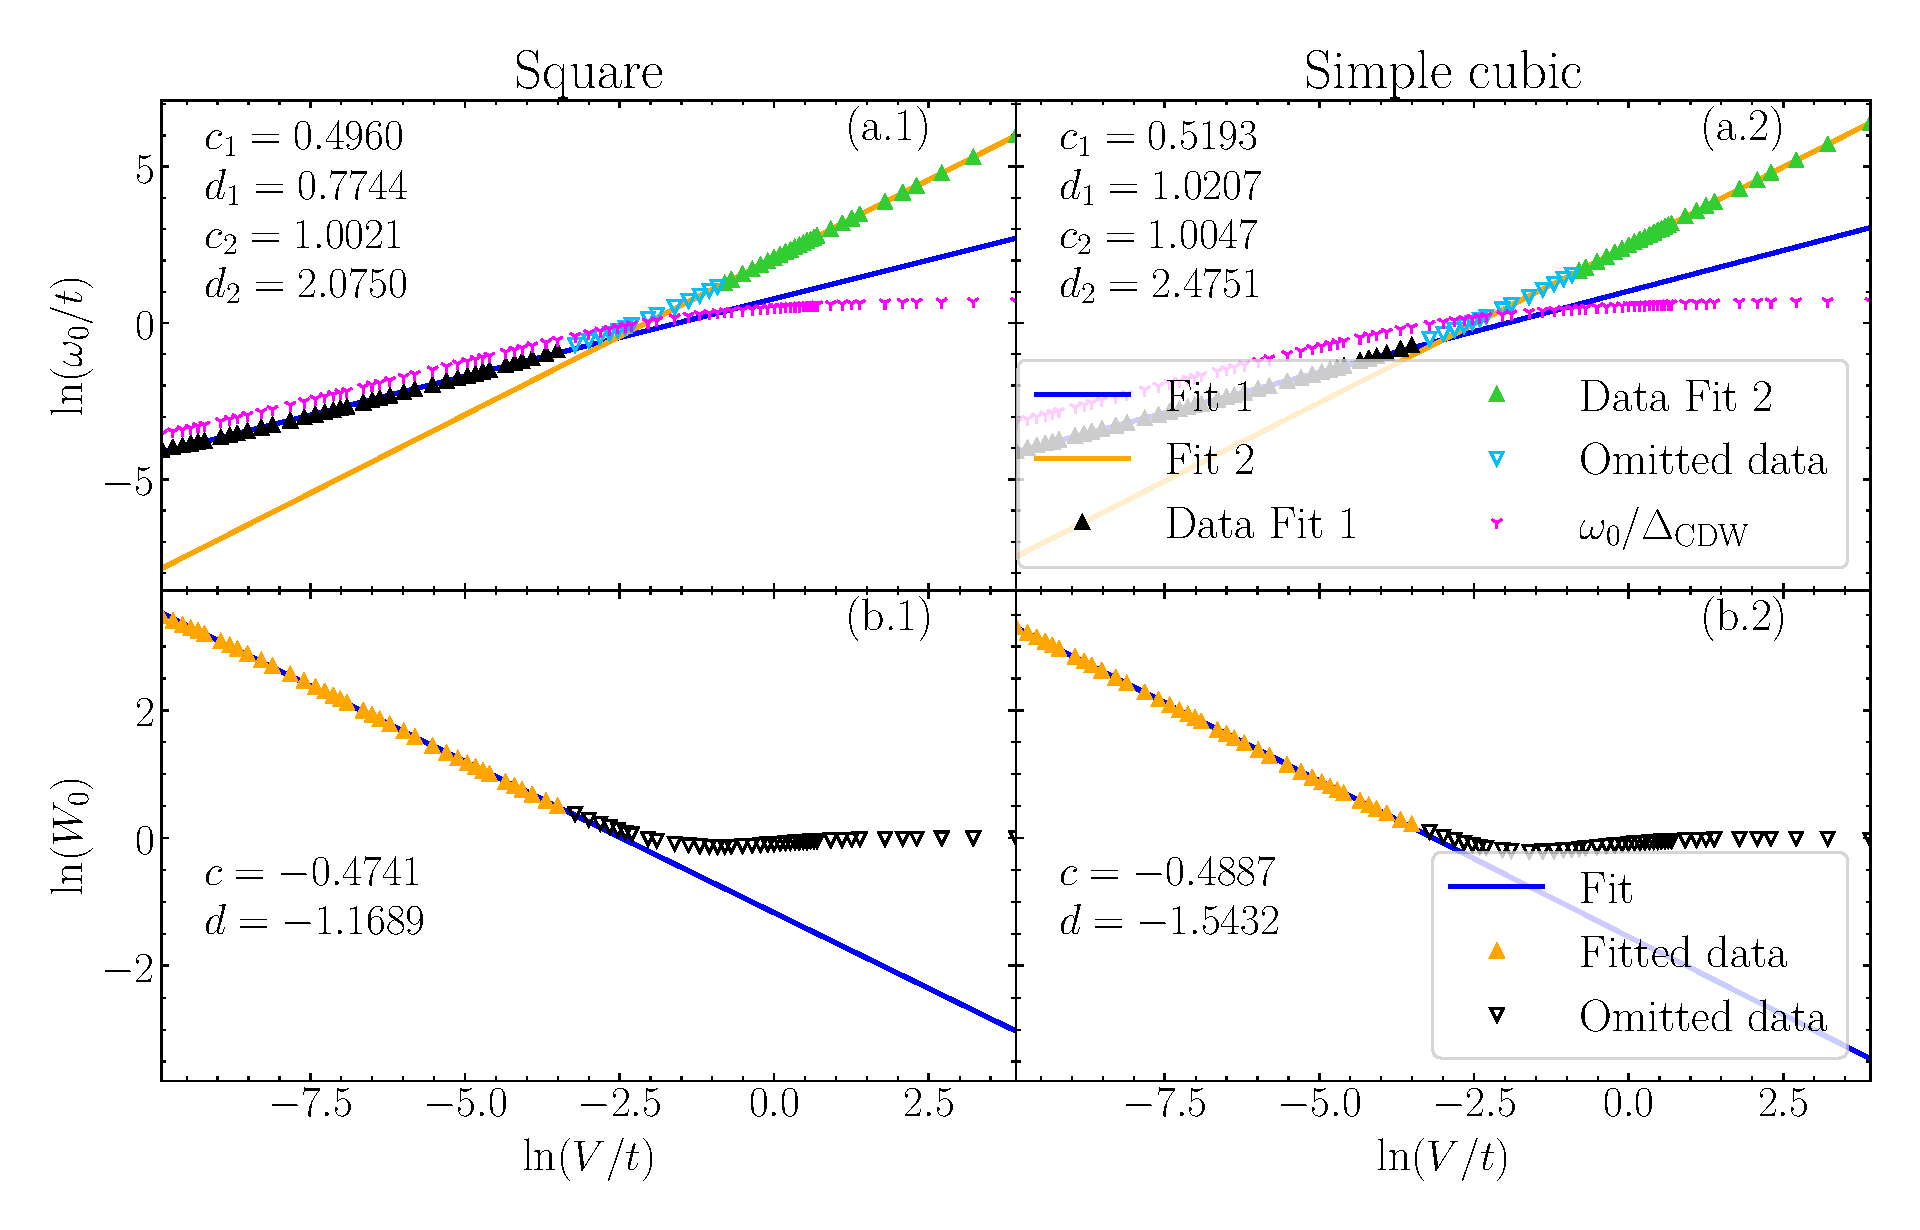
\includegraphics[width=\textwidth]{plots/sc_peak_in_cdw.pdf} % NV sketch
    \center{\textcolor{tudarkgreen}{Weight and position of the peak in the SC spectral functions in the CDW phase.}}
\end{minipage}
\hfill
\begin{minipage}{0.49\textwidth}
    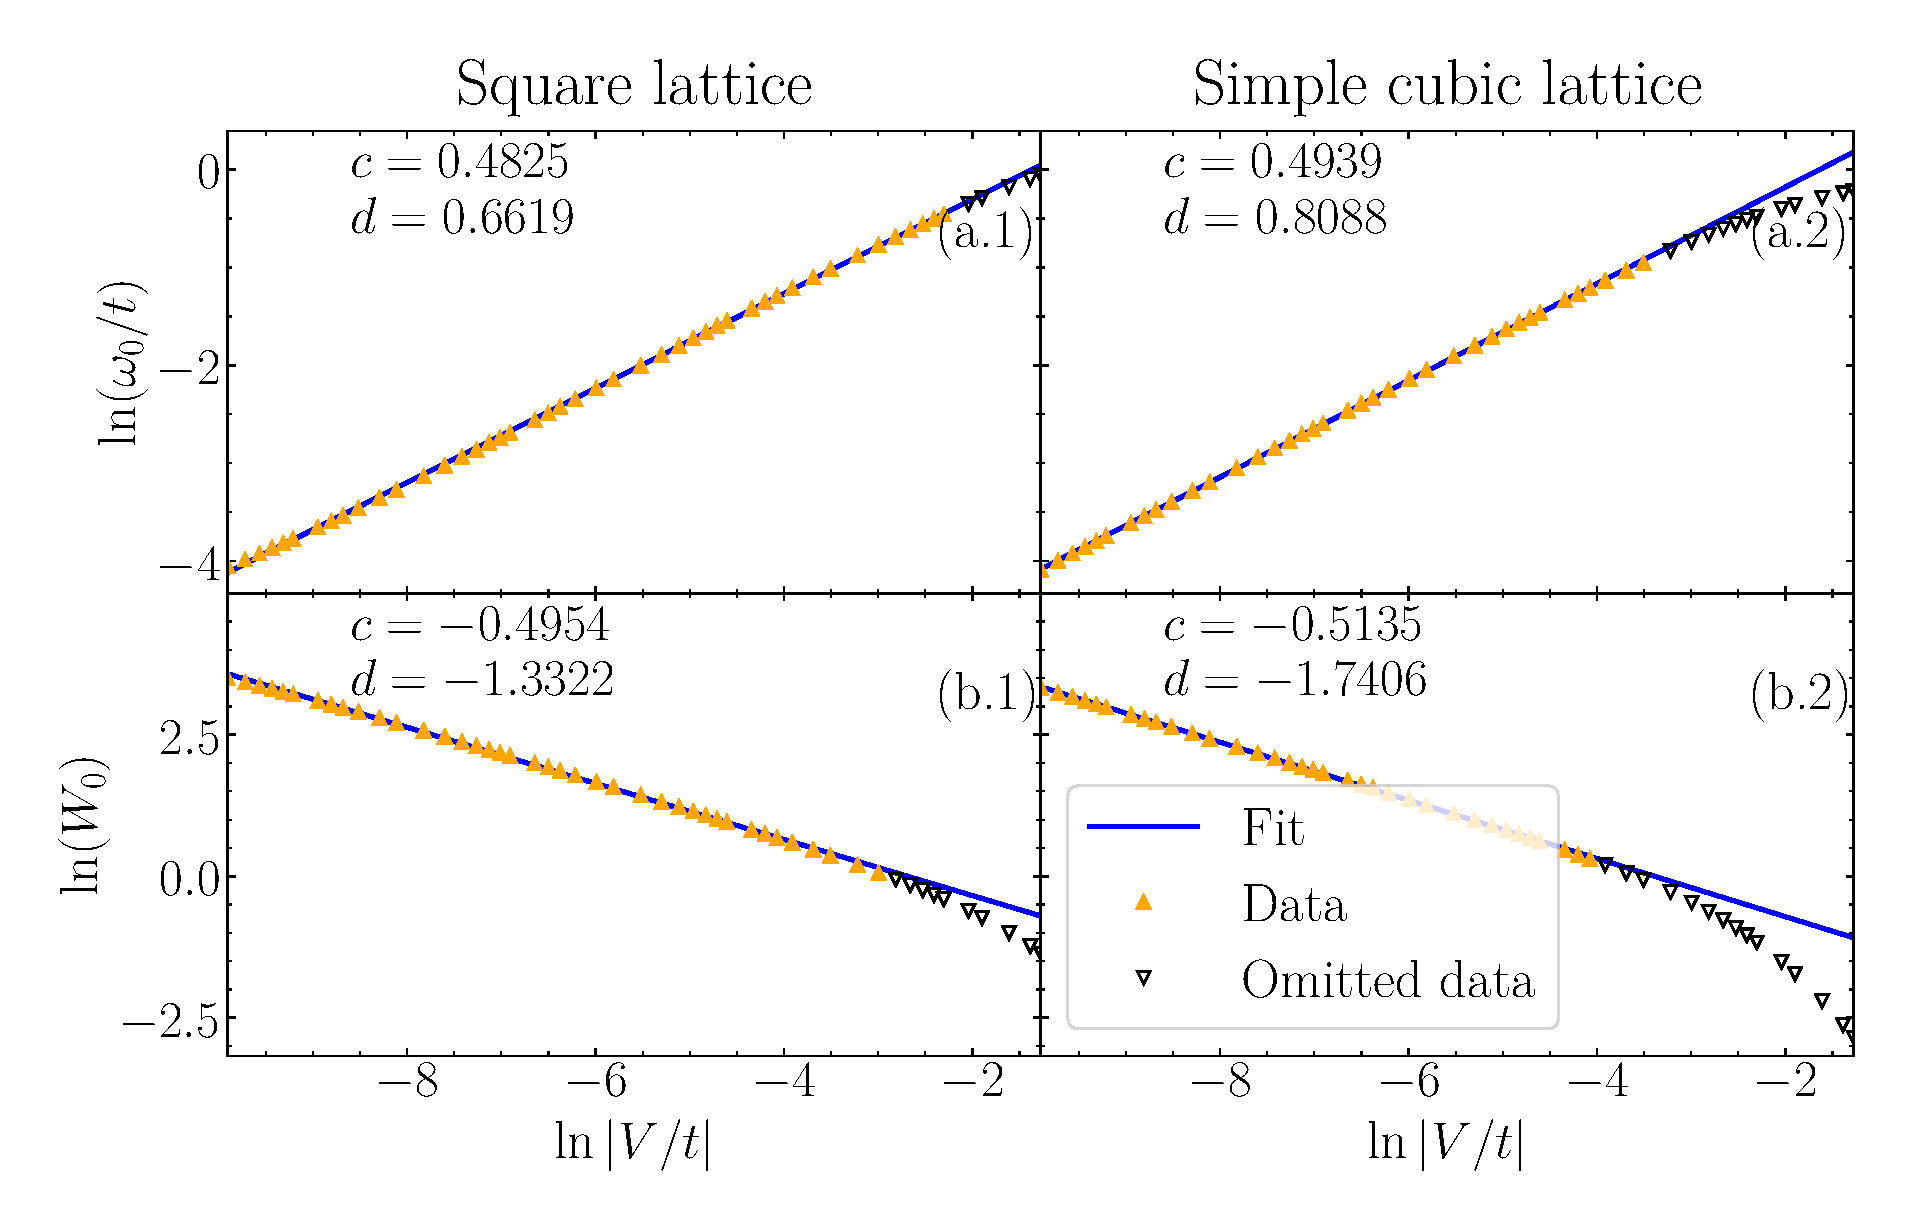
\includegraphics[width=\textwidth]{plots/cdw_peak_in_sc.pdf} % NV sketch
    \center{\textcolor{tudarkgreen}{Weight and position of the peak in the CDW spectral functions in the SC phase.}}
\end{minipage}
\begin{itemize}
    \item Double-logarithmic plots
    \item The weights diverge as $1/\sqrt{|V|}$ while the peak positions move to $0$ as $\sqrt{|V|}$
    \item For $V\gg t$, the weights become constant. The position grows linearly and the position in units of the gap becomes constant.
\end{itemize}

\begin{minipage}{0.49\textwidth}
    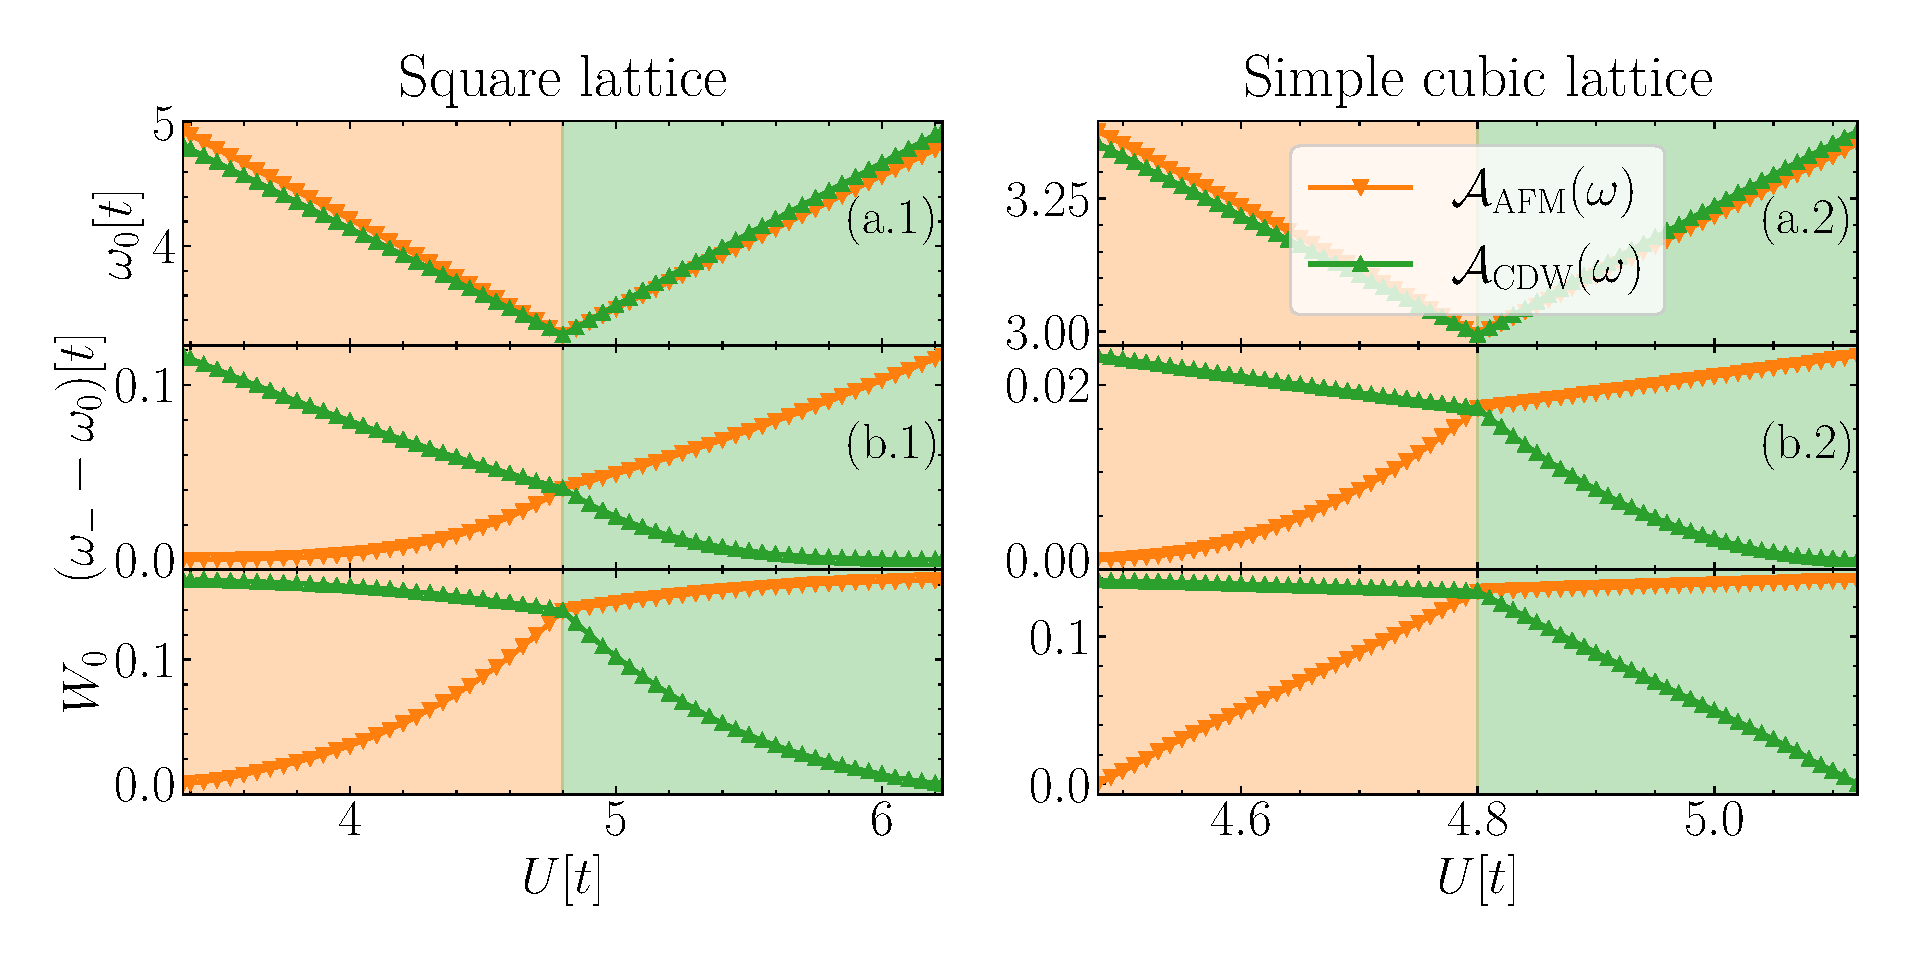
\includegraphics[width=\textwidth]{plots/afm_cdw_peaks_overview.pdf} % NV sketch
    \center{\textcolor{tudarkgreen}{Weight and position of the peak in the AFM and CDW spectral functions close to the phase transition.}}
\end{minipage}
\hfill
\begin{minipage}{0.49\textwidth}
    \begin{itemize}
        \item Orange region: System is in the CDW phase, blue region: System is in the AFM phase
        \item Peak position grows linearly with $U$ as the system moves away from the phase transition
        \item But it moves into the continuum (b) quadratically
        \item At the same time, the weights also vanish
    \end{itemize}
\end{minipage}

}


\posterbox{2cm}{106cm}{38cm}{Possible outlook}
{%
\begin{itemize}
\item Incorporating phase-separated states into the mean-field theory, thereby providing deeper analysis of the negative $V$ regime of phase diagrams and collective excitations
\item Coupling the electronic system to the electromagnetic field to include the Anderson-Higgs mechanism for superconductors
\item Describing multi-band systems with even richer phases and collective excitations
\end{itemize}
}

\posterbox{42cm}{110cm}{38cm}{References}
{%
\begingroup
\renewcommand{\section}[2]{}	% for removing the bibliography title
\begin{thebibliography}{99}
    %\begin{multicols}{2}
    \bibitem{Kalthoff17} M. Kalthoff, F. Keim, H. Krull, and G. S. Uhrig, The European Physical Journal B 90, 97 (2017).
    \bibitem{Bleicker18} P. Bleicker and G. S. Uhrig, Phys. Rev. A 98, 033602 (2018).
    \bibitem{Micnas88b} R. Micnas, J. Ranninger, S. Robaszkiewicz, and S. Tabor, Phys. Rev. B 37, 9410 (1988).
    \bibitem{Linner23} E. Linnér, C. Dutreix, S. Biermann, and E. A. Stepanov, Phys. Rev. B 108, 205156 (2023).
    %\end{multicols}          
\end{thebibliography}
\endgroup
}

% Do not remove this, for the sake of archeology!
\node [anchor=north] at ($(\paperwidth-1cm,.9cm-\paperheight)$) {\tiny \the\year};
\end{tikzpicture}

\end{document}

